\documentclass[10pt,twocolumn]{article}
\usepackage[top=19mm,bottom=19mm,left=20mm,right=20mm,columnsep=1cm]{geometry}
\usepackage{mathptmx}
\usepackage[T1]{fontenc}
\usepackage{graphicx,booktabs,amsmath,caption,titlesec,enumitem}
\usepackage[hidelinks]{hyperref}
\captionsetup{font=small,labelfont=bf}
\titleformat{\section}{\normalfont\small\bfseries\scshape\centering}{\Roman{section}.}{0.5em}{}
\titleformat{\subsection}{\normalfont\small\itshape}{\Alph{subsection}.}{0.5em}{}
\titlespacing*{\section}{0pt}{8pt}{4pt}
\titlespacing*{\subsection}{0pt}{5pt}{2pt}
\setlist{nosep,leftmargin=*}
\renewcommand{\thesection}{\Roman{section}}
\begin{document}
\twocolumn[{
\begin{center}
{\LARGE Night Physiology, Latent Recovery, and Mood:\\ A State Space Analysis of Raw Fitbit Data in LifeSnaps}\\[6pt]
{\normalsize Maitrey Phatak}\\
{\small University of Florida, EEE6778 Applied Machine Learning II, Project Deliverable 2}\\
{\small m.phatak@ufl.edu \quad \url{https://github.com/maittreyyyy/lifesnaps-recovery-ssm}}\\[8pt]
\end{center}
\noindent\small\textbf{\textit{Abstract}.} This preliminary report documents the first full implementation of a pipeline that extracts intraday physiology from the raw LifeSnaps Fitbit export, estimates latent recovery states with state space models, relates them to self reported mood, and exposes the results in an interactive Streamlit explorer. From 9.1\,GB of raw records the pipeline builds 2{,}338 cleaned nights from 57 participants with heart rate every 5\,s, HRV every 5\,min, sleep stage timelines, and wrist temperature. A three state Kalman model selected by BIC separates autonomic strain, the within night trajectory, and sleep fragmentation; only autonomic strain persists across days (half life about 0.6 days). Across six analyses with held out evaluation, none of these states improves mood prediction beyond mood history and the person's own baseline (best balanced accuracy 0.357 for seven classes, chance 0.143).
\vspace{10pt}}]

\section{Project Summary}
The project asks whether nightly physiological recovery, measured by a consumer wearable, explains how people report feeling the next day. Deliverable 1 established the repository, a data audit, and a Stage 1 linear state space model on the daily LifeSnaps CSV summaries \cite{lifesnaps}. That model produced a plausible latent recovery state but no reliable gain in mood prediction, matching an independent LifeSnaps benchmark \cite{gavai}.

Since Deliverable 1 the project moved from daily summaries to the raw intraday export, which prior LifeSnaps analyses did not use; the closest prior work relates sleeping heart rate curve shape to mental health with a different device and cohort \cite{fudolig}. Implemented since then: (1) extraction of 48.7M heart rate, 220k HRV, 4.4M wrist temperature records and 4{,}141 sleep logs into Parquet; (2) a documented cleaning funnel; (3) ten night features per night; (4) four model families with held out evaluation; (5) an interactive explorer that replays nights one morning at a time. Remaining work: confidence intervals, leave one subject out evaluation, a learned night encoder, and the live wearable connection.

\section{System Architecture and Pipeline}
Fig.~\ref{fig:arch} shows the data flow. The raw BSON export is streamed once into columnar Parquet files and queried with DuckDB, which reduces any later query from a 3 minute scan to seconds. Cleaning and feature extraction run as SQL over the Parquet files. The models run in NumPy and SciPy. A single export step writes per day states, mood reports, and fitted parameters, which the Streamlit interface loads.

\begin{figure}[t]
\centering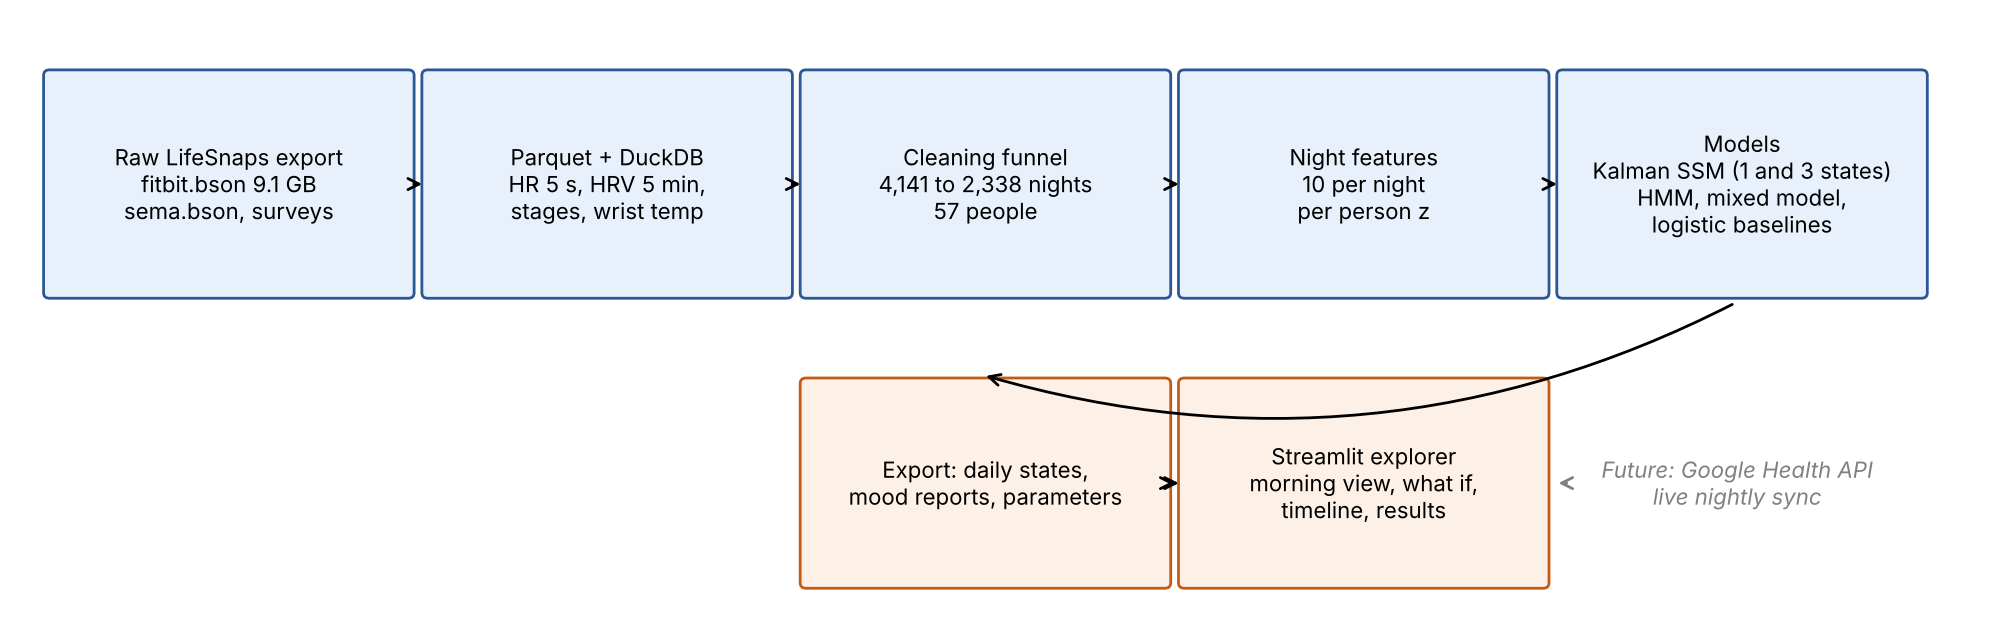
\includegraphics[width=\linewidth]{architecture_d2.png}
\caption{Pipeline from the raw export to the interface. The grey element is future work.}
\label{fig:arch}
\end{figure}

\textbf{Data.} LifeSnaps \cite{lifesnaps} contains 71 participants from Greece, Cyprus, Italy and Sweden who wore a Fitbit Sense in two rounds (May 24 to Jul 26 2021, $n{=}38$; Nov 15 2021 to Jan 17 2022, $n{=}34$; one person in both). The raw export holds 32 Fitbit data types and 73M records. Sampling intervals were measured, not assumed: heart rate median 5\,s (90th percentile 15\,s), HRV exactly 300\,s during sleep, wrist temperature 60\,s. Signal coverage per night is bimodal by person (Table~\ref{tab:cov}).

\begin{table}[h]
\centering\small
\caption{Share of main sleep nights with each signal (69 people)}
\label{tab:cov}
\begin{tabular}{lccc}\toprule
Signal & Median & 25th pct. & People at 0\%\\\midrule
Heart rate & 100\% & 100\% & 0\\
HRV (5 min) & 87\% & 0\% & about 26\\
Sleep stages & 95\% & 88\% & about 8\\
Wrist temperature & 96\% & 90\% & about 9\\\bottomrule
\end{tabular}
\end{table}

\textbf{Cleaning.} Nights pass five steps (Table~\ref{tab:funnel}): main sleep only; 180 to 900 minutes asleep; one night per date (longest kept); and the person's mood reporting window, following the rules of a public LifeSnaps multilevel analysis \cite{multilevel}. Mood reports outside the seven valid categories (8 reports) are removed. Reports before 06:00 link to the previous night.

\begin{table}[h]
\centering\small
\caption{Cleaning funnel}
\label{tab:funnel}
\begin{tabular}{lrr}\toprule
Step & Nights & People\\\midrule
All sleep records & 4{,}141 & 69\\
Main sleep only & 3{,}688 & 69\\
180 to 900 min asleep & 3{,}562 & 65\\
One night per date & 3{,}431 & 65\\
Inside mood window & 2{,}338 & 57\\\bottomrule
\end{tabular}
\end{table}

\textbf{Night features.} From 5\,min median heart rate: nadir, nadir timing as a fraction of the night, and the drop from the first 10\% to 20 to 30\% of the night. From HRV: mean RMSSD and late minus early RMSSD. From stages: deep fraction, share of deep sleep in the first half, wake bouts per hour. Mean wrist temperature and minutes asleep complete the set. Features are z scored within person and clipped at $\pm4$.

\section{Model Implementation Details}
\textbf{Recovery state space model.} For person $i$ on day $t$,
\begin{align*}
\mathbf{x}_t &= \Phi\,\mathbf{x}_{t-1} + B\,\mathbf{u}_t + \mathbf{w}_t, & \mathbf{w}_t&\sim\mathcal{N}(0,Q)\\
\mathbf{y}_t &= C\,\mathbf{x}_t + \mathbf{v}_t, & \mathbf{v}_t&\sim\mathcal{N}(0,R)
\end{align*}
with inputs $\mathbf{u}_t$ = (sleep minutes, previous day steps), observations $\mathbf{y}_t$ = nine night features, and in the extended model also daily valence and arousal derived from the mood categories with a circumplex mapping. $\Phi$ and $R$ are diagonal, $Q=I$, and $C$ is lower triangular to fix rotation. Missing observations are skipped in the Kalman update. Parameters are fitted by maximum likelihood (L-BFGS-B), vectorized across all people; the number of states (1 to 3) is chosen by BIC. Mood on each person's last 30\% of days is hidden during fitting and predicted one step ahead.

\textbf{Hidden Markov model.} A discrete alternative: each day sits in one of $K$ regimes with Gaussian physiology and a categorical distribution over the seven moods, fitted with Baum Welch EM in log space; $K\in\{1..5\}$ by BIC.

\textbf{Per person coupling.} A linear mixed model, valence$_t$ = $a_i$ + $s_i x_t$ + $c\,$valence$_{t-1}$, with a random slope $s_i$ per person on the recovery state.

\textbf{Baselines.} Carry forward, and class balanced multinomial logistic regression on time of day and previous mood, with nightly averages, night features, or the recovery state added.

\textbf{Setup and reproducibility.} Python 3.10 on UF HiPerGator (Open OnDemand Jupyter, 16\,GB, 4 cores); DuckDB 1.x, pandas, NumPy, SciPy, scikit learn, statsmodels. Conversion takes about 3 minutes; the three state fit 85\,s; the HMM sweep under 3 minutes. All analysis choices sit in one decisions cell of \texttt{notebooks/lifesnaps\_analysis.ipynb}; the notebook was verified end to end on a synthetic dataset with the same schema, where the HMM recovered a planted recovery to mood link.

\section{Interface Prototype}
The Streamlit recovery tracker (\texttt{ui/app.py}) is written for a person tracking their own recovery and replays one participant one morning at a time, as a syncing watch would (Fig.~\ref{fig:ui}). The strain state is shown as a recovery score, $100(1-\Phi(\text{strain}))$, where 50 is the person's usual night, with plain labels (well recovered, about usual, under recovered). \textbf{Input:} person, morning, and two plan sliders (tonight's sleep and today's activity, from much less to much more than usual). \textbf{Output:} the score with change from yesterday, plain comparisons of overnight heart rate, HRV, disruption and sleep length, a short advice line, tomorrow's expected score under the plan, the day's mood check ins, and a trend view of the score with short nights and mood (Fig.~\ref{fig:ui2}); model details sit in a separate tab, regimes and mood with short nights marked, and the evaluation tables. \textbf{Usability:} each view uses only nights up to the selected morning, the plan sliders expose the fitted dynamics in everyday terms, and technical terms are confined to the How it works tab. \textbf{Limitations:} the night detail view (raw 5\,min signals) is not yet included; forecasts use population parameters; the explorer deliberately shows mood next to physiology rather than forecasting it, because the evaluation does not support a mood forecast.

\begin{figure}[t]
\centering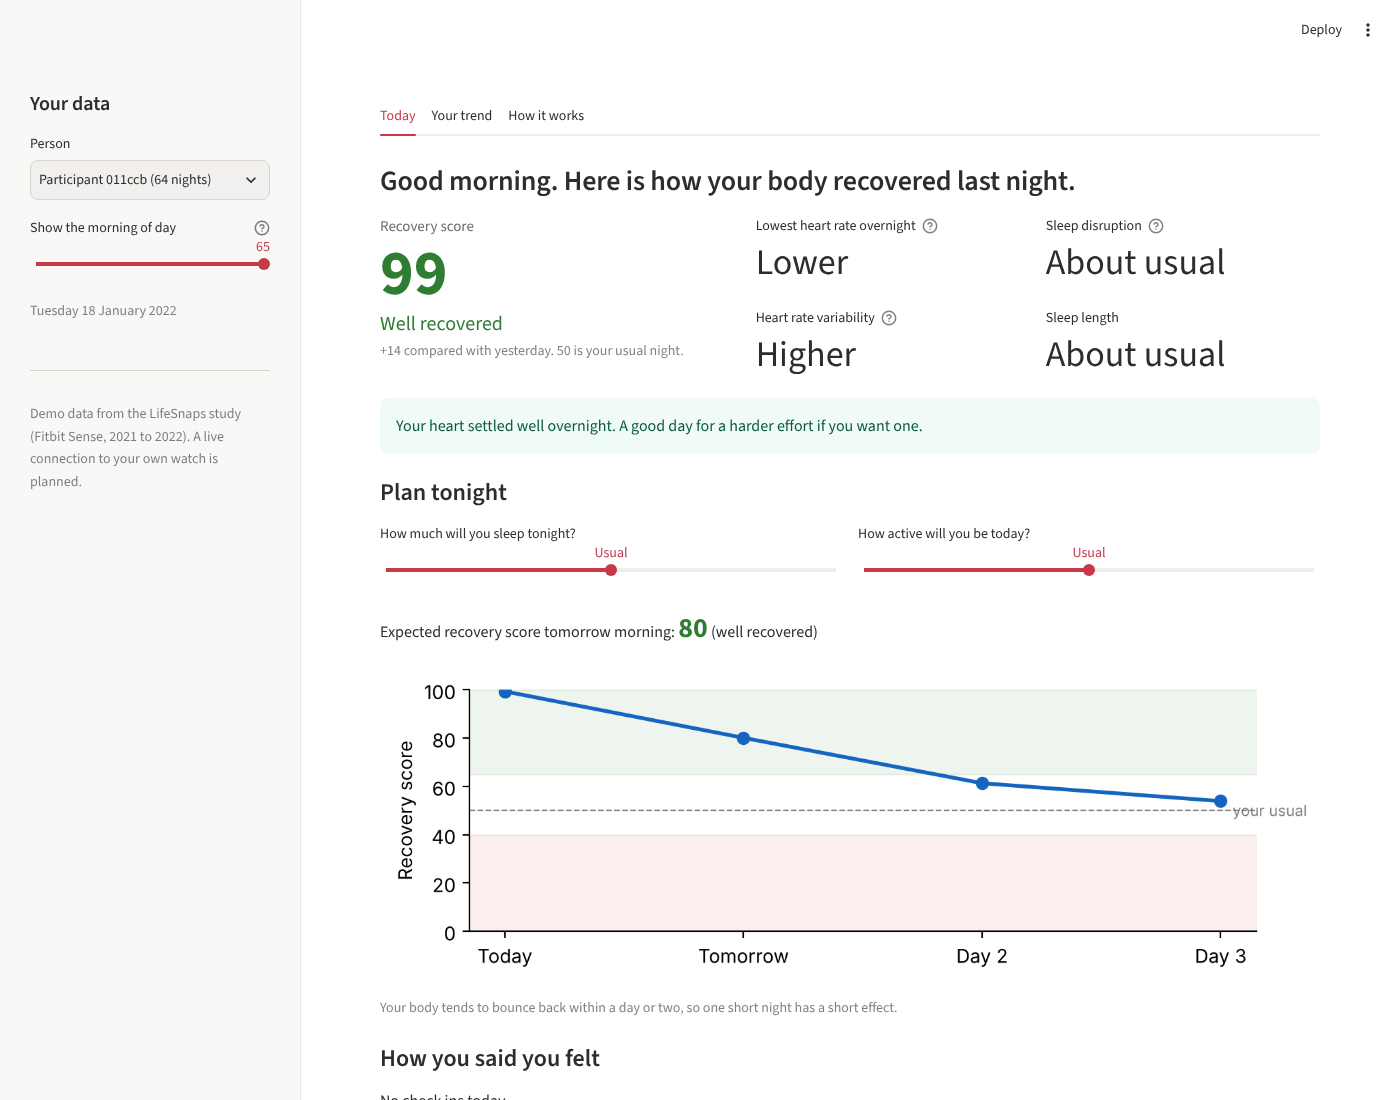
\includegraphics[width=\linewidth]{ui_morning.png}
\caption{Recovery tracker, morning view: score, plain comparisons, and the plan for tonight.}
\label{fig:ui}
\end{figure}


\begin{figure}[t]
\centering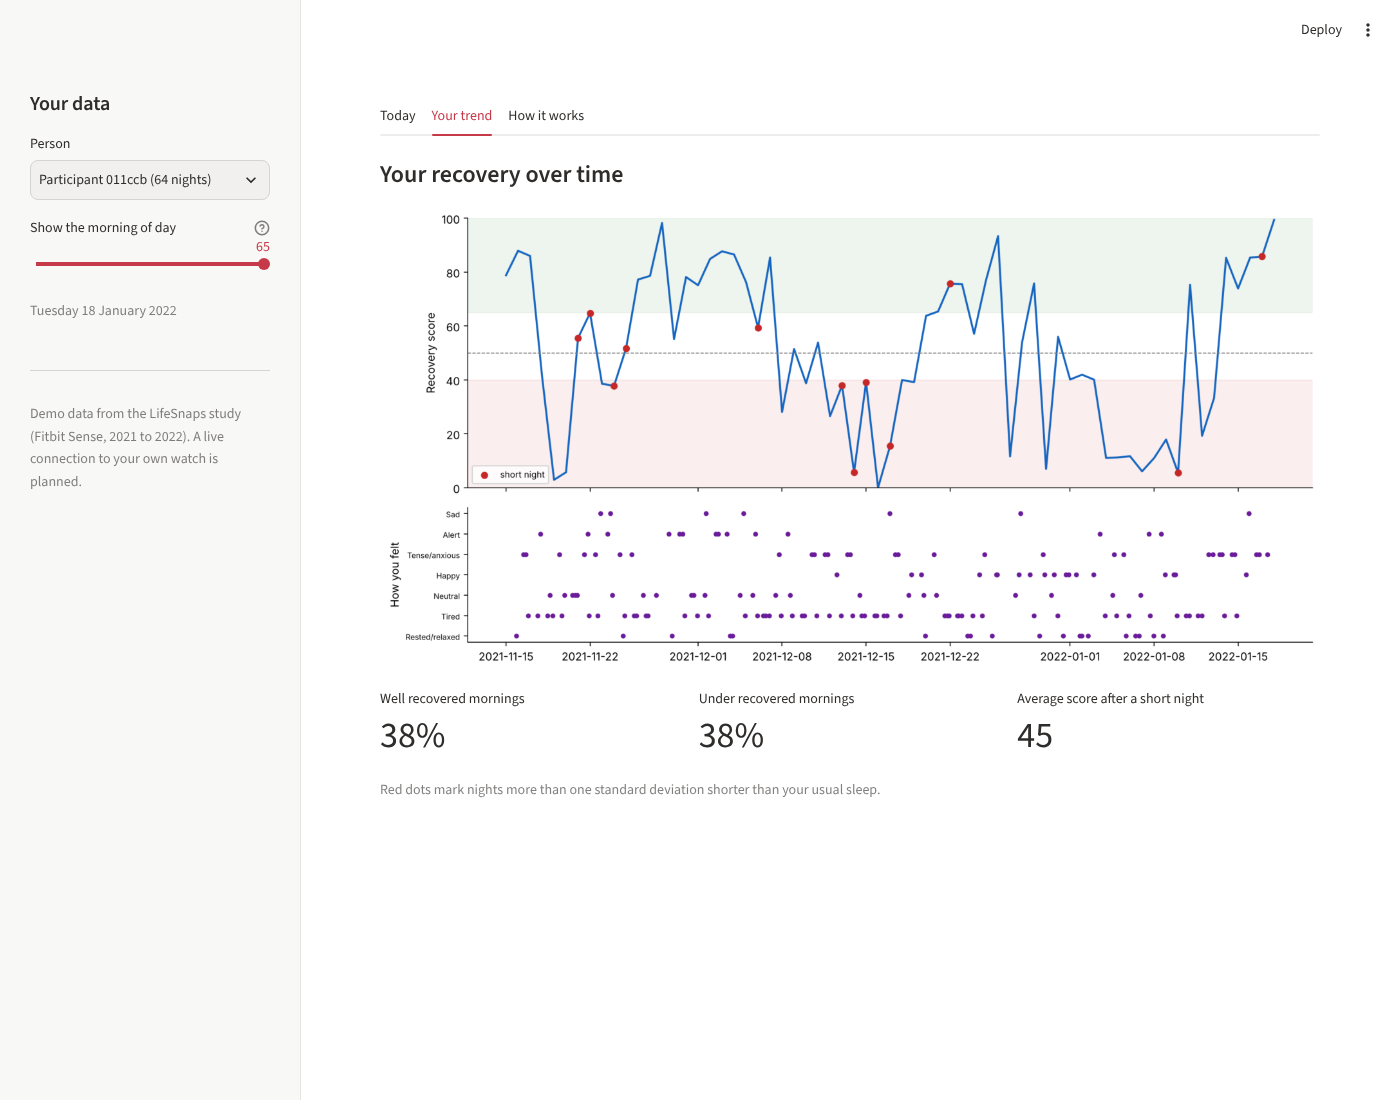
\includegraphics[width=\linewidth]{ui_timeline.png}
\caption{Recovery tracker, trend view: recovery score over time with short nights marked, and mood check ins.}
\label{fig:ui2}
\end{figure}

\section{Early Evaluation and Results}
\textbf{Physiology responds to sleep.} On 331 short nights (sleep more than 1 SD below the person's usual), heart rate nadir rises by 0.49 SD and RMSSD falls by 0.33 SD relative to the same person's other nights (Fig.~\ref{fig:short}). Count based features (wake bouts, deep minutes) scaled with night length and were converted to rates.

\begin{figure}[t]
\centering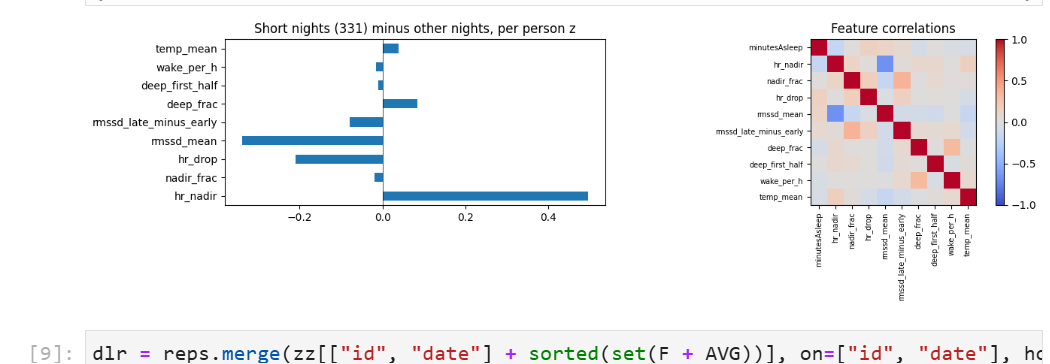
\includegraphics[width=\linewidth]{short_nights.png}
\caption{Short nights minus other nights (per person z) and feature correlations.}
\label{fig:short}
\end{figure}

\textbf{Hidden states.} The one state model reduces to an autonomic factor (nadir loading fixed at $-1$, RMSSD $+0.79$; other features load below 0.2) with $\phi=0.37$, a half life of 0.7 days; sleep raises it ($+0.16$) and previous day steps lower it ($-0.13$). BIC selects three states (BIC 61{,}570, 61{,}352, 61{,}199 for 1, 2, 3 states), shown in Table~\ref{tab:states}. The state dips on the day of a short night and returns to baseline the next day (Fig.~\ref{fig:rec}), unlike the five day persistence of the Stage 1 model built on Fitbit's daily resting heart rate; whether that persistence reflects smoothing in the daily summary is an open question.

\begin{table}[h]
\centering\small
\caption{Three state model: main loadings and persistence}
\label{tab:states}
\begin{tabular}{p{1.65cm}p{3.1cm}p{1.65cm}}\toprule
State & Main loadings & $\phi$ (half life)\\\midrule
Strain & HR nadir $+0.87$, RMSSD $-0.63$ & 0.34 (0.6 d)\\
Unfolding & nadir timing $-0.54$, RMSSD late minus early $-0.58$ & 0.05\\
Fragmentation & wake per hour $+0.89$, deep fraction $+0.35$ & 0.05\\\bottomrule
\end{tabular}
\end{table}

\begin{figure}[t]
\centering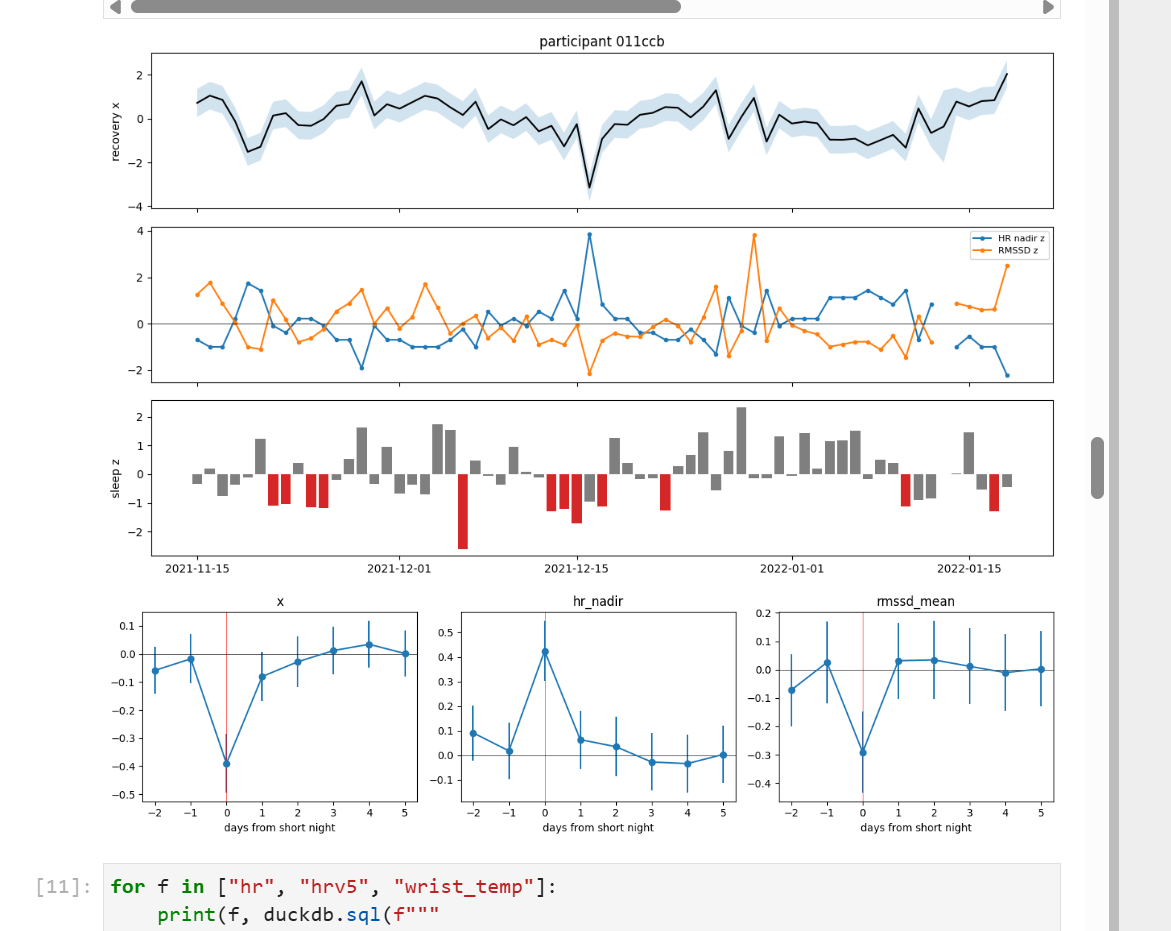
\includegraphics[width=\linewidth]{recovery_event.png}
\caption{Top: recovery state with $\pm2$ SD band, nightly HR nadir and RMSSD, and sleep (short nights red) for one participant. Bottom: mean response around short nights with 95\% CI.}
\label{fig:rec}
\end{figure}

\textbf{Mood.} Table~\ref{tab:mood} lists held out results (1{,}505 test reports, 49 people). Physiology changes balanced accuracy by $-0.016$ to $+0.001$. In the three state model, valence and arousal load at most 0.04 on any state (noise 0.96), and one step predictions equal the person mean (valence RMSE 1.027 for both). The HMM (best $K=5$) matches the population mood frequencies (log loss 1.79 against 1.794), while each person's own frequencies reach 1.559. In the mixed model the average slope of valence on recovery is 0.006 (95\% CI $-0.06$ to 0.07), the between person slope variance is 0.009 (SE 0.010), and no person slope exceeds 0.2 in magnitude; previous day valence is the only significant predictor (0.13, $p<.001$).

\begin{table}[h]
\centering\small
\caption{Held out seven class mood prediction}
\label{tab:mood}
\begin{tabular}{lcc}\toprule
Model & Bal.\ acc. & Macro F1\\\midrule
Carry forward & 0.357 & 0.356\\
Time + previous mood & 0.352 & 0.304\\
+ nightly averages & 0.348 & 0.314\\
+ night features & 0.341 & 0.304\\
+ recovery state & 0.353 & 0.306\\
+ state + night features & 0.343 & 0.305\\\bottomrule
\end{tabular}
\end{table}


\begin{table}[h]
\centering\small
\caption{HMM regimes ($K{=}5$): physiology means (per person z) and most likely moods}
\label{tab:hmm}
\begin{tabular}{p{0.5cm}p{3.2cm}p{2.9cm}}\toprule
Reg. & Physiology & Mood (probability)\\\midrule
S1 & strain: nadir $+0.54$, RMSSD $-0.58$ & neutral .30, tired .24\\
S2 & strain, steps $+0.38$ & tired .29, rested .23\\
S3 & recovered: nadir $-0.83$, RMSSD $+0.85$ & tired .24, rested .17, tense .17\\
S4 & near usual & rested .40, happy .20\\
S5 & deep $+2.75$, wake $+3.13$ (1 day) & artifact nights\\\bottomrule
\end{tabular}
\end{table}

\begin{table}[h]
\centering\small
\caption{Stage 1 (Deliverable 1) against the raw data models}
\label{tab:cmp}
\begin{tabular}{p{2.2cm}p{2.5cm}p{2.3cm}}\toprule
& Stage 1, daily CSV & D2, raw intraday\\\midrule
Observations & resting HR, nightly RMSSD & 9 night features (+ mood)\\
States & 1 & 3 (BIC)\\
Persistence & $\phi{=}0.87$, 5.1 d & $\phi{=}0.34$, 0.6 d\\
Mood gain & $+0.004$ & $+0.001$\\\bottomrule
\end{tabular}
\end{table}

Table~\ref{tab:hmm} summarizes the HMM regimes and Table~\ref{tab:cmp} contrasts the Stage 1 model with the raw data models.

\textbf{Interpretation.} The models function: they recover sensible physiology, respond to sleep and activity in the expected directions, and on synthetic data recover a planted link. On LifeSnaps, mood is explained by its own history and by person level baselines, not by the night. The HMM also isolated a one day regime with deep fraction $+2.75$ SD and wake rate $+3.13$ SD, which identifies corrupt sleep records.

\section{Challenges and Next Steps}
\textbf{Challenges.} (1) Data volume: the 9.1\,GB export required a streaming conversion and a columnar store. (2) Per person missingness: HRV is present on about 90\% of nights for 43 people and absent for the rest, so missingness is a property of the device or person, not the night. (3) Raw data quality: 134{,}133 duplicate heart rate rows, 98{,}586 readings with confidence 0, and a few nights with deep sleep above total sleep. (4) Study timing: data extends outside the two official rounds, including one participant who recorded continuously from May 2021 to January 2022; the mood window rule handles this.

\textbf{Before Deliverable 3.} Participant bootstrap confidence intervals and leave one subject out evaluation; a learned encoder over the 5\,min night sequence compared with the hand made features; mood predicting the next night (reverse direction); PANAS and STAI, measured about six times per person, as slower outcomes; a night detail view in the interface; and a Google Health API connector design, since the Fitbit Web API was turned off in October 2026 \cite{ghapi}.

\section{Responsible AI Reflection}
\textbf{Privacy.} LifeSnaps is anonymized and released under CC BY 4.0; the app stores only participant codes, dates, z scores and mood labels. A live connection would require Google's restricted scope review beyond 100 users \cite{ghapi}. \textbf{Fairness.} The cohort is 71 adults from four European countries who wore one device model; parameters may not transfer to other populations or devices. \textbf{Trust.} Because the evidence does not support a mood forecast, the interface shows mood next to physiology and states the null result, rather than presenting a confident prediction. \textbf{Misuse.} The states are research estimates, not clinical measures.

\begin{thebibliography}{9}\small
\bibitem{lifesnaps} S. Yfantidou et al., ``LifeSnaps, a 4 month multi modal dataset capturing unobtrusive snapshots of our lives in the wild,'' \emph{Scientific Data}, vol. 9, 663, 2022.
\bibitem{gavai} A. Gavai and J. Heringa, ``When do learned representations improve longitudinal health prediction? A persistence anchored, information matched benchmark of wearable data and personalized models,'' Zenodo, 2026.
\bibitem{fudolig} M. I. Fudolig et al., ``The two fundamental shapes of sleep heart rate dynamics and their connection to mental health in college students,'' \emph{Digital Biomarkers}, 2024.
\bibitem{multilevel} L. Xu, ``lifesnaps-multilevel-public,'' GitHub repository, github.com/lizxu-byte/lifesnaps-multilevel-public, accessed Nov. 2026.
\bibitem{ghapi} Google, ``About the Google Health API,'' developers.google.com/health/about, accessed Nov. 2026.
\end{thebibliography}
\end{document}
